\documentclass[tikz,border=2pt]{standalone}
\usepackage{amsmath,amssymb}
\usepackage{pgfplots}
\pgfplotsset{compat=1.18}

\begin{document}
% The partial derivative with respect to x_1 at x0: freeze x_2 = b, so the surface is cut by the
% plane x_2 = b into a curve, and differentiate that one-variable curve at x_1 = a.
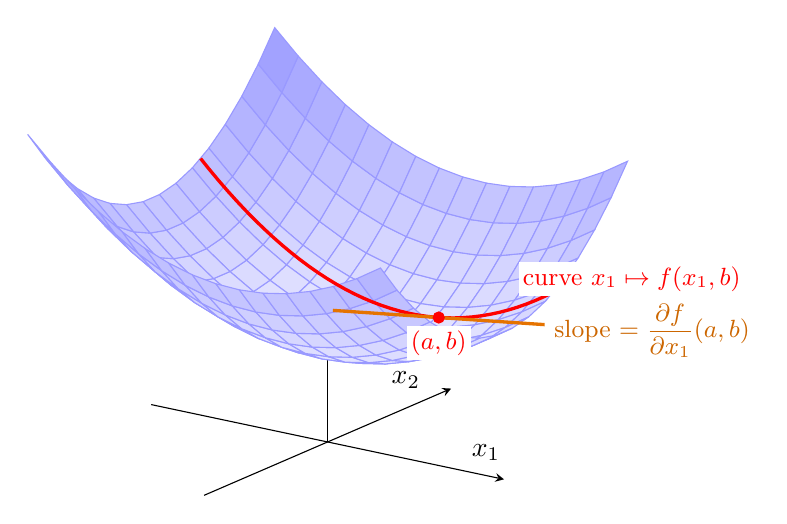
\begin{tikzpicture}
	\begin{axis}[
		view={35}{28},
		xmin=-2, xmax=2, ymin=-2, ymax=2, zmin=0, zmax=5,
		xlabel={$x_1$}, ylabel={$x_2$}, zlabel={},
		xtick=\empty, ytick=\empty, ztick=\empty,
		axis lines=center, clip=false,
		width=9.2cm, height=7cm
		]
		% surface z = 2 + 0.4 x1^2 + 0.6 x2^2 - 0.3 x1
		% flat shading only: dvisvgm drops the mesh shadings that interp shaders produce
		\addplot3[surf, shader=faceted, faceted color=blue!40, colormap={pale}{color=(blue!8) color=(blue!40)}, samples=16, domain=-2:2, domain y=-2:2, z buffer=sort] {2+0.4*x^2+0.6*y^2-0.3*x};
		% the slice x2 = b = 0.8
		\addplot3[red, very thick, samples=40, samples y=0, domain=-2:2] (x, 0.8, {2+0.4*x^2+0.6*0.64-0.3*x});
		% the point x0=(a,b)=(0.7,0.8): z = 2+0.196+0.384-0.21 = 2.37 ; slope dz/dx1 = 0.8*0.7-0.3 = 0.26
		\addplot3[only marks, mark=*, mark size=2pt, red] coordinates {(0.7,0.8,2.37)};
		\addplot3[orange!90!black, very thick, samples=2, samples y=0, domain=-0.5:1.9] (x, 0.8, {2.37+0.26*(x-0.7)});
		\node[red, anchor=west, font=\small, fill=white, inner sep=1.5pt] at (axis cs:1.6,0.8,3.5) {curve $x_1\mapsto f(x_1,b)$};
		\node[orange!80!black, anchor=west, font=\small] at (axis cs:1.9,0.8,2.55) {slope $=\dfrac{\partial f}{\partial x_1}(a,b)$};
		\node[red, anchor=north, font=\small, fill=white, inner sep=1.5pt] at (axis cs:0.7,0.8,2.2) {$(a,b)$};
	\end{axis}
\end{tikzpicture}
\end{document}
